\documentclass[10pt,a4paper]{report}
\usepackage[utf8]{inputenc}
\usepackage{amsmath}
\usepackage{amsfonts}
\usepackage{amssymb}
\usepackage{graphicx}

\usepackage{hyperref}

\usepackage{float}
\usepackage{multicol}
\usepackage{xhfill}

\usepackage{comment}

\begin{document}
	\begin{center}
		\textbf{{\Large EXERCÍCIO 1}
		\\
		{\normalsize Implementar e treinar o modelo Adaline para reconhecer os símbolos A e A invertida}}
	\end{center}

	\section{Dados}
	
	\begin{figure*}[h]
		\centering
		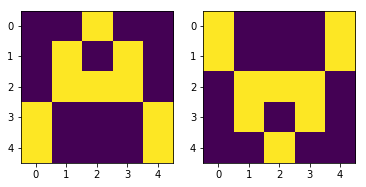
\includegraphics[width=4cm, height=2cm]{patterns.png}
		\caption{Patterns}
		\label{fig:patterns}
	\end{figure*}

	\begin{figure*}[h]
		\centering
		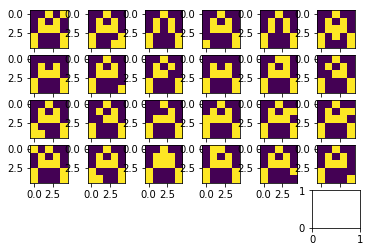
\includegraphics[width=9cm, height=5cm]{a_normal.png}
		\caption{Samples , Normal A's}
		\label{fig:patterns}
	\end{figure*}

	\begin{figure*}[h]
		\centering
		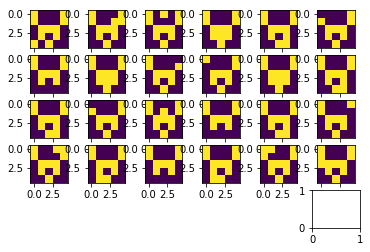
\includegraphics[width=9cm, height=5cm]{a_inverted.png}
		\caption{Samples , Inverted A's}
		\label{fig:patterns}
	\end{figure*}
	
	All this data was created using \href{https://nbviewer.jupyter.org/github/jahirmedinacs/usp-2018-2_IRNA/blob/master/Aula\%201/exe1/Data.ipynb}{\textbf{THIS}} juypter notebook (Python Conda Kernel)
	
	\section{ADALINE Perceptron}
	
	\subsection{Note}
	\textbf{{\large \href{https://nbviewer.jupyter.org/github/jahirmedinacs/usp-2018-2_IRNA/blob/master/Aula\%201/exe1/exc1.ipynb}{\textbf{THIS}} juypter notebook (Python Conda Kernel) is the script use for training , test and construction of the perceptron.}}
	
	\subsection{Considerations}
	
	\begin{itemize}
		\item Being the data binary, but written in a no common manner (using -1 and 1) could be transformed to in a regular representation (0 and 1), but by specifications of this exercise, every operation has to be operated using -1 and 1.
		\item When weights are generated, is used a random function; this random function creates values between 0 and 1, its possible to extend this range multiplying for some scalar, but, knowing the data set is linearly separable and also posses a binary data format, the right choice is to keep the 0 to 1 range
	\end{itemize}

	\subsection{ADALINE}
	
	The ADALINE learning method uses the delta rule (this is not other than the gradient operator) as weight re-adjust technique; it's true in the ADALINE model, the adjustment ratio isn't dynamic but isn't necessary because the perceptron can only classify Linearly Separable Sets, Binary Class specifically
	\\
	\\
	That static value who works as adjustment ratio is called "Teacher",  choose the right value for this constant is important, because, if its choose wrong could create a no convergence stated (if exist a global minimum, the adjustment step for reach it is bigger than the necessary, bypassing it).
	\\
	\\
	Like can be viewed in the code, not only is important choose correctly the teacher value, is necessary to use at least the right minimal amount of \textit{epochs}, if it's lower than necessary the training process never converge, if it's bigger than necessary you have been wasted computer power, time and possibly generated an \textit{over-fitting}
	\\
	\\
    Finally, later of the training process, during the testing process (using $70\%$ of the data for training and $30\%$ for testing) is possible to verify that, even when the values are near to the expected, some values are very distant.
	\\
	\\
	But, we have the certainty that the data is binary,  when some value is bigger than 0, no matter the value, is 1, and when is less than 0,  became -1.
	\\
	\\
	Remembering, Remaining, that last "value correction" is made because, using values like [-1, 1] generates some erratics result, but keeping the sign.
	


\end{document}

